\documentclass{article}
\usepackage[preprint,nonatbib]{neurips_2026}
\usepackage[T1]{fontenc}
\usepackage{amsmath,amssymb,graphicx,booktabs,hyperref}
\setlength{\intextsep}{7pt}
\hypersetup{hidelinks,pdftitle={Painting Generation with a DCGAN},pdfauthor={Hongyi Ding}}
\makeatletter
\renewcommand{\@noticestring}{ECE 285: Deep Generative Models, Homework 2, Fall 2026.}
\makeatother
\newcommand{\ValFIDA}{0.0950}
\newcommand{\ValISA}{2.90}
\newcommand{\ValFIDB}{0.0706}
\newcommand{\ValISB}{3.64}
\newcommand{\ValFIDC}{0.0918}
\newcommand{\ValISC}{2.81}
\newcommand{\ValFIDD}{0.0992}
\newcommand{\ValISD}{1.95}
\newcommand{\TestFID}{0.0830}
\newcommand{\TestIS}{3.64}
\newcommand{\RealValFID}{0.0355}
\newcommand{\RealTestFID}{0.0410}
\newcommand{\RealTestIS}{5.51}
\newcommand{\RoneHundredFID}{0.1247}

\title{Painting Generation with a DCGAN}
\author{Hongyi Ding \quad {\normalfont UC San Diego}\\
{\footnotesize\textbf{Code: }\href{https://github.com/mafeifei798/ece285-hw2-wikiart-gan}{\nolinkurl{github.com/mafeifei798/ece285-hw2-wikiart-gan}}}}
\begin{document}
\maketitle
\begin{abstract}
This report compares four DCGAN configurations for generating WikiArt paintings.
A wider model with horizontal flips and averaged generator weights gave the best
result after 200 epochs: test probability FID \TestFID{} and IS \TestIS{}.
The samples capture varied colors and compositions, but faces and objects remain distorted.
\end{abstract}

\section{Data and model}
The data consists of 12,000 randomly sampled \href{https://www.kaggle.com/datasets/steubk/wikiart}{WikiArt images}.
After removing 12 duplicates, 9,988 images were used for training and 1,000 each
for validation and testing. All 27 styles are included. Images were resized
with their aspect ratio preserved, center-cropped to $128\times128$ RGB, and
scaled to $[-1,1]$. This kept training manageable. Style labels were not used.

The generator maps $z\sim\mathcal N(0,I_{128})$ to $4\times4$ features and upsamples
five times with transposed convolutions, BatchNorm and ReLU, ending in Tanh.
The discriminator uses strided convolutions, BatchNorm and LeakyReLU (0.2).
Non-saturating training minimizes real-plus-fake binary cross-entropy (BCE)
for the discriminator and BCE against real labels for the generator.

\section{Training configurations}
All runs used Adam ($lr=2\times10^{-4}$, betas 0.5/0.999), batch size 64 and
seed 2026, with one discriminator update per generator update.
I ran a width-32 baseline for 100 epochs, then three width-64 models for 200:
\begin{itemize}
\setlength\itemsep{0pt}
\item \textbf{R1:} width 64, horizontal flips, and generator exponential moving
average (EMA), decay 0.999.
\item \textbf{R2:} R1 plus differentiable color, translation and cutout augmentation
of real and generated discriminator inputs.
\item \textbf{R3:} R2 plus nearest-neighbor/conv upsampling, discriminator spectral
normalization replacing BatchNorm, and hinge loss replacing BCE.
\end{itemize}


\begin{figure}[h!]
\centering
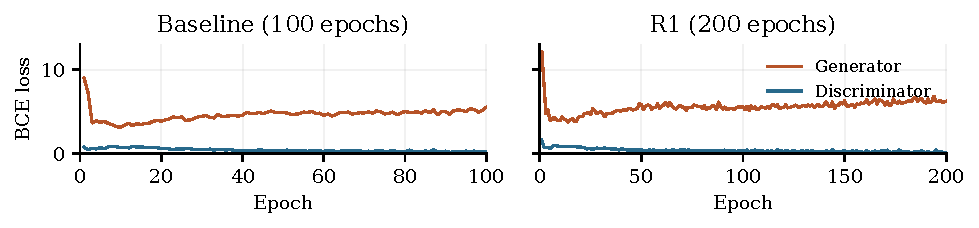
\includegraphics[width=\linewidth]{figures/losses.pdf}
\caption{Generator and discriminator losses averaged over each epoch. The curves use
the training weights; R1's sample evaluation uses EMA weights.}
\label{fig:loss}
\end{figure}

\newpage
\section{Results and observations}
Evaluation used Ignite 0.5.4 and the assignment tutorial\footnote{\url{https://pytorch-ignite.ai/blog/gan-evaluation-with-fid-and-is/}},
with 1,000 real and 1,000 generated images per comparison. Both were converted
to 8-bit RGB and resized bilinearly to $299\times299$.
FID is computed from 1,000-dimensional Inception class probabilities.
Its numerical scale is much smaller than that of the usual 2,048-feature FID,
so the two scores are not directly comparable.
IS is computed over the full generated set. Every checkpoint uses the same noise
vectors, making the sample comparisons easier to follow.

\begin{table}[h!]
\centering
\small
\begin{tabular}{llrrr}
\toprule
Split & Configuration & Epoch & FID $\downarrow$ & IS $\uparrow$\\
\midrule
Validation & Baseline (raw) & 100 & \ValFIDA & \ValISA\\
 & R1 (EMA) & 200 & \textbf{\ValFIDB} & \textbf{\ValISB}\\
 & R2 (EMA) & 180 & \ValFIDC & \ValISC\\
 & R3 (EMA) & 160 & \ValFIDD & \ValISD\\
\midrule
Test & Selected R1 (EMA) & 200 & \TestFID & \TestIS\\
\bottomrule
\end{tabular}
\caption{Best validation checkpoints and the final test result. R1 uses the same generated
images for validation and test, so its IS is the same in both rows.}
\label{tab:results}
\end{table}

I compared checkpoints from R1--R3 at epoch 1 and every 20 epochs, using
validation FID to choose the final model. R1 at epoch 200 came out best, so
I used its EMA weights for the test evaluation. The extra augmentation in R2
and the combination of changes in R3 both gave worse scores.

R1 needed the longer run to overtake the baseline. At epoch 100, its validation
FID was \RoneHundredFID{}, versus \ValFIDA{} for the baseline; by epoch 200,
it had dropped to \ValFIDB{}. The improvement includes both the model changes
and the extra 100 epochs of training.

\begin{figure}[h!]
\centering
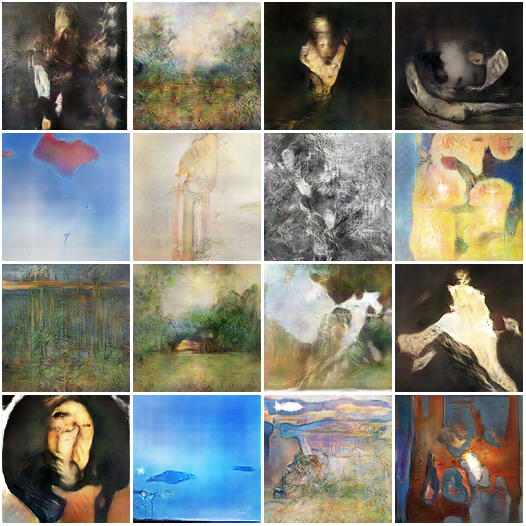
\includegraphics[width=.51\linewidth]{figures/generated.png}
\caption{The first 16 generated images from the final evaluation, in sampling order.
Each image is $128\times128$.}
\label{fig:samples}
\end{figure}

One thing I noticed was that generator loss did not track sample quality.
It rose after an early drop, while validation FID improved later in training.
R1 ended with discriminator loss 0.084 and generator loss 6.25
(Figure~\ref{fig:loss}), yet epoch 200 had its lowest validation FID.
Choosing a checkpoint by generator loss alone would have missed this result.

Looking at the samples, the model has learned more about color and composition
than object shape. There are landscape-like scenes, portraits and abstract
textures, but many faces and boundaries look distorted. Real train images
versus real test images scored FID \RealTestFID{}, and real test images had
IS \RealTestIS{}. R1 was the best of the runs tried here; drawing coherent
objects remains the clearest weakness in its samples.
\end{document}
